% ============================================================================
% MÓDULO 3 — CAPÍTULO 8
% Morfopedologia e Processos Interativos Relevo–Solo–Água (Semana 8)
% ============================================================================

\chapter{Morfopedologia e Processos Interativos Relevo–Solo–Água}
\label{cap:morfopedologia}

\noindent\tagEmenta\ \tagPratica

\begin{capObjetivos}
Ao concluir este capítulo (Semana 8 do Plano CHF662), você será capaz de:
\begin{enumerate}[leftmargin=1.6em, itemsep=2pt]
  \item Explicar os fundamentos da \textbf{abordagem morfopedológica} (Guerra, 2018; Casseti, 2007; Ross, 2006) e a interdependência genética entre formas de vertente, rocha, água e distribuição de solos ao longo de uma \textbf{topossequência}.
  \item Calcular a \textbf{declividade de vertentes} em porcentagem ($S\%$) e em graus ($\theta$), tanto diretamente no terreno quanto a partir de cartas topográficas ou medições de distância inclinada, e classificá-la segundo os sistemas da \textbf{EMBRAPA} e de \textbf{Ross}.
  \item Analisar o papel regulador da cobertura vegetal no balanço entre infiltração e escoamento superficial, relacionando-o à gênese de processos erosivos e ao assoreamento de fundos de vale.
  \item Diferenciar os principais tipos de \textbf{movimentos de massa} (rastejo, escorregamento rotacional, escorregamento translacional, corrida de detritos/lama e queda de blocos) quanto à velocidade, geometria, gatilhos e sinais diagnósticos em campo.
\end{enumerate}
\end{capObjetivos}

\begin{capRevisao}
Para aproveitar integralmente este capítulo, conecte três elementos já consolidados:
\begin{itemize}[leftmargin=1.5em, itemsep=2pt]
  \item \textbf{Vertentes como subsistemas da bacia (Cap. 7):} toda bacia hidrográfica é composta por vertentes que drenam para os canais; é sobre essas encostas que a chuva incide primeiro, definindo quanto infiltrará e quanto escoará carregando sedimentos.
  \item \textbf{Noções básicas de trigonometria em triângulos retângulos:} em uma encosta inclinada, o desnível vertical ($\Delta h$) é o cateto oposto ao ângulo de inclinação $\theta$, a distância horizontal ($d_h$) é o cateto adjacente e a distância inclinada ao longo do terreno ($d_{\text{inc}}$) é a hipotenusa, de modo que $\tan\theta = \Delta h / d_h$ e $d_{\text{inc}}^2 = \Delta h^2 + d_h^2$.
  \item \textbf{Escala cartográfica:} em uma carta de escala $1:E$, cada $1\text{ cm}$ no mapa corresponde a $E\text{ cm}$ no terreno (por exemplo, na escala 1:25.000, $1\text{ cm}$ equivale a $25.000\text{ cm} = 250\text{ m}$).
\end{itemize}
\end{capRevisao}

\etapa{3}{Explicação Teórica — Abordagem Morfopedológica, Vertentes, Declividade e Movimentos de Massa}

\begin{boxSimbolo}[Vocabulário Técnico e Símbolos do Capítulo 8]
\begin{itemize}[leftmargin=1.4em, itemsep=2.5pt]
  \item \textbf{Morfopedologia:} método integrado de análise da paisagem que estuda conjuntamente a morfogênese (formas do relevo e processos geomorfológicos), a litologia e a pedogênese (formação e distribuição espacial dos solos).
  \item \textbf{Vertente (encosta):} superfície inclinada que conecta o divisor de águas (interflúvio) ao fundo de vale, composta por segmentos de diferentes curvaturas e declividades.
  \item \textbf{Topossequência (ou catena):} sucessão lateral de solos distintos que se desenvolvem do topo à base de uma mesma vertente em função das variações de relevo, drenagem interna e transporte de materiais.
  \item \textbf{Colúvio:} depósito de solo e fragmentos de rocha transportados vertente abaixo pela gravidade e pelo escoamento difuso, acumulando-se geralmente no sopé côncavo.
  \item \textbf{Desnível vertical ($\Delta h$):} diferença de altitude entre o ponto mais alto e o ponto mais baixo de um segmento de vertente ($\Delta h = H_2 - H_1$), em metros ($\text{m}$).
  \item \textbf{Distância horizontal ($d_h$):} projeção horizontal entre dois pontos da vertente (distância medida em planta ou carta topográfica), em metros ($\text{m}$).
  \item \textbf{Distância inclinada ($d_{\text{inc}}$):} comprimento real percorrido sobre a superfície inclinada do terreno (medido com trena ao longo da rampa), em metros ($\text{m}$).
  \item \textbf{Declividade ($S\%$ e $\theta$):} inclinação da vertente expressa em porcentagem ($S\%$) ou em graus sexagesimais ($\theta^\circ$).
  \item \textbf{Poropressão ($u$):} pressão exercida pela água acumulada nos poros do solo; quando positiva e elevada, reduz o atrito entre grãos e diminui a estabilidade da encosta.
\end{itemize}
\end{boxSimbolo}

\section{A Abordagem Morfopedológica: Relevo, Solo e Água em Interação}

Historicamente, a Geomorfologia (ciência das formas de relevo) e a Pedologia (ciência dos solos) desenvolveram-se muitas vezes em compartimentos separados. A \textbf{abordagem morfopedológica}, consolidada no Brasil por autores como \textbf{Castro e Salomão (2000)}, \textbf{Casseti (2007)}, \textbf{Ross (2006)} e \textbf{Guerra (2018)} a partir das contribuições francesas de Tricart e Kilian, rompe essa separação ao demonstrar que \textbf{o relevo e o solo evoluem simultaneamente sob a ação da água e da gravidade}.

Na prática da Análise Ambiental, a morfopedologia parte de um princípio direto: a geometria da vertente governa o caminho da água (se ela infiltra verticalmente ou escoa lateralmente), e esse regime hídrico governa a espessura, a textura, o grau de intemperismo e a estabilidade do solo. Em contrapartida, as propriedades do solo (porosidade, coesão, profundidade e mudança textural entre horizontes) condicionam a resistência do terreno à erosão e aos deslizamentos, moldando de volta o perfil da vertente.

\section{Formas de Vertente e Distribuição de Solos (Topossequência)}

Uma vertente típica raramente é uma rampa reta e uniforme. Ao caminhar do divisor de águas até o leito do rio, o geógrafo observa cinco setores morfopedológicos característicos, integrados na Figura~\ref{fig:morfopedologia_vertente} e detalhados na Tabela~\ref{tab:topossequencia}:

\begin{enumerate}[leftmargin=1.6em, itemsep=2.5pt]
  \item \textbf{Topo plano ou suave (interflúvio):} declividade muito baixa, energia do escoamento superficial reduzida e amplo predomínio da \textbf{infiltração vertical}. A água percola profundamente, favorecendo o intemperismo químico intenso e a formação de solos profundos, bem drenados e envelhecidos, como os \textbf{Latossolos} (típicos dos tabuleiros e chapadões baianos).
  \item \textbf{Ombro convexo (alta vertente):} a declividade começa a aumentar progressivamente para jusante. O fluxo superficial ganha velocidade e inicia-se o transporte seletivo de partículas finas (erosão laminar e rastejo). Os solos tornam-se gradualmente menos espessos.
  \item \textbf{Meia encosta retilínea (média vertente):} segmento mais inclinado da vertente, onde predomina a transferência rápida de água e sedimentos (zona de transporte/erosão). A taxa de remoção superficial aproxima-se ou supera a taxa de formação do solo, originando solos rasos, pedregosos e jovens, como \textbf{Neossolos Litólicos} e \textbf{Cambissolos}. É o setor mais suscetível a sulcos, ravinas e escorregamentos.
  \item \textbf{Sopé côncavo (baixa vertente / pedimento):} a declividade volta a diminuir, desacelerando o escoamento superficial e subsuperficial. Ocorre deposição de sedimentos coluviais vindos de montante e concentração de umidade em subsuperfície, favorecendo a formação de \textbf{Argissolos} (com acúmulo de argila no horizonte B) e \textbf{Planossolos} (comuns nas depressões sertanejas, sujeitos a adensamento subsuperficial e encharcamento sazonal).
  \item \textbf{Fundo de vale (planície fluvial / várzea):} relevo plano junto ao canal fluvial, com lençol freático raso e deposição periódica de aluviões. Desenvolvem-se solos hidromórficos (\textbf{Gleissolos}) ou jovens aluviais (\textbf{Neossolos Flúvicos}). Quando as vertentes a montante são degradadas, este setor recebe o excesso de sedimentos, sofrendo \textbf{assoreamento}.
\end{enumerate}

\begin{figure}[H]
  \centering
  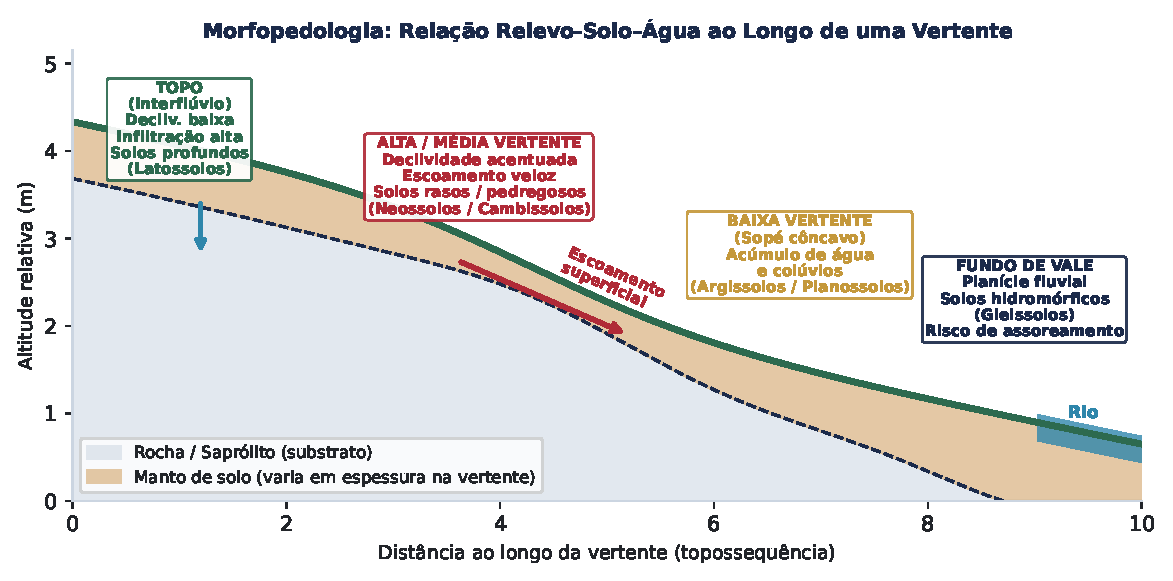
\includegraphics[width=0.94\textwidth]{figures/fig06_morfopedologia_vertente.pdf}
  \caption{Perfil morfopedológico integrado de uma vertente (topossequência), evidenciando a variação da espessura do manto de solo, do balanço infiltração/escoamento e das classes pedológicas do topo ao fundo de vale.}
  \label{fig:morfopedologia_vertente}
\end{figure}

\begin{table}[H]
\centering
\caption{Relação genética entre setores da vertente, dinâmica hídrica, classes de solos e susceptibilidade ambiental.}
\label{tab:topossequencia}
\renewcommand{\arraystretch}{1.20}
\small
\begin{tabularx}{\textwidth}{@{}p{2.3cm} p{2.2cm} p{2.9cm} p{2.7cm} >{\raggedright\arraybackslash}X@{}}
  \toprule
  \rowcolor{uefsNavy}
  \textcolor{white}{\bfseries Setor da Vertente} & \textcolor{white}{\bfseries Forma / Declividade} & \textcolor{white}{\bfseries Dinâmica Hídrica Dominante} & \textcolor{white}{\bfseries Solos Típicos (SiBCS)} & \textcolor{white}{\bfseries Fragilidade / Processo Principal} \\
  \midrule
  Topo (interflúvio) & Plano a suave ($< 8\%$) & Infiltração vertical intensa & Latossolos (profundos) & Baixa erosão natural; sensível à compactação agrícola. \\
  \rowcolor{bgGray}
  Ombro (alta vertente) & Convexo ($8\text{--}20\%$) & Aceleração do escoamento difuso & Latossolos / Argissolos & Erosão laminar e início de sulcos em solo exposto. \\
  Meia encosta & Retilíneo íngreme ($> 20\%$) & Escoamento veloz e remoção ativa & Neossolos Litólicos e Cambissolos & Alta fragilidade: ravinas e movimentos de massa. \\
  \rowcolor{bgGray}
  Sopé (baixa vertente) & Côncavo ($3\text{--}12\%$) & Convergência de fluxos e coluvionamento & Argissolos e Planossolos & Erosão em ravinas/voçorocas por fluxo subsuperficial. \\
  Fundo de vale & Plano ($< 3\%$) & Saturação hídrica e inundação & Gleissolos e Neossolos Flúvicos & Assoreamento do canal e inundações sazonais. \\
  \bottomrule
\end{tabularx}
\end{table}

\section{Declividade da Vertente: Cálculo e Classificação (EMBRAPA e Ross)}

A \textbf{declividade} é o principal parâmetro quantitativo que expressa a energia gravitacional atuante sobre uma encosta. Quanto maior a declividade, maior é a componente tangencial da gravidade que acelera o escoamento superficial e solicita o solo ao cisalhamento (deslizamento). Na Geografia e na Engenharia Ambiental, a declividade é expressa de duas maneiras complementares: em \textbf{porcentagem ($S\%$)} e em \textbf{graus ($\theta$)}.

\begin{boxFormula}[Declividade de Vertentes em Porcentagem ($S\%$) e em Graus ($\theta$)]
\textbf{Origem e finalidade:} derivada da trigonometria do triângulo retângulo formado pela projeção horizontal e pelo desnível vertical do terreno, a declividade quantifica o grau de inclinação de uma rampa para fins de mapeamento pedológico (EMBRAPA), análise de fragilidade ambiental (Ross, 1994), planejamento urbano e aplicação do Código Florestal (encostas com $\theta > 45^\circ$, ou $S > 100\%$, são APPs).

\textbf{Equações fundamentais:}
\[
  S(\%) = \frac{\Delta h}{d_h} \times 100 \qquad\text{e}\qquad \theta = \arctan\!\left(\frac{\Delta h}{d_h}\right)
\]
\textbf{Relações auxiliares indispensáveis em Geografia:}
\begin{itemize}[leftmargin=1.5em, itemsep=1.5pt]
  \item \textbf{A partir de carta topográfica (escala $1:E$):} se a distância medida no mapa entre duas curvas de nível é $d_{\text{mapa}}$ (em metros ou convertida de cm para m), então $d_h = d_{\text{mapa}} \times E$.
  \item \textbf{A partir de trena no terreno (distância inclinada $d_{\text{inc}}$):} pelo Teorema de Pitágoras, obtém-se primeiro a distância horizontal:
  \[
    d_h = \sqrt{d_{\text{inc}}^2 - \Delta h^2}.
  \]
  \item \textbf{Conversão direta entre graus e porcentagem:} $S(\%) = 100 \cdot \tan\theta$ e $\theta = \arctan(S / 100)$.
\end{itemize}

\textbf{Variáveis e unidades:} $\Delta h$ e $d_h$ devem estar obrigatoriamente na \textbf{mesma unidade de comprimento} (ambos em metros, por exemplo).

\textbf{Exemplo numérico completo:} uma encosta desce da cota $316\text{ m}$ para a cota $280\text{ m}$ ao longo de uma distância horizontal de $d_h = 200\text{ m}$.
\begin{align*}
  \Delta h &= 316 - 280 = 36\text{ m} \\
  S(\%) &= \frac{36}{200} \times 100 = 0,18 \times 100 = 18,0\% \\
  \theta &= \arctan(0,18) \approx 10,20^\circ.
\end{align*}
\textbf{Interpretação:} a cada $100\text{ m}$ percorridos na horizontal, o terreno sobe ou desce $18\text{ m}$. Pelas classes da Tabela~\ref{tab:classes_declividade}, o relevo é \textbf{Ondulado} (EMBRAPA) e apresenta \textbf{Fragilidade Média — Classe 3} (Ross, 1994).
\end{boxFormula}

Note um marco conceitual que elimina erros em provas: \textbf{uma declividade de $45^\circ$ corresponde exatamente a $100\%$}, pois $\tan(45^\circ) = 1$, o que significa que $\Delta h = d_h$ (o terreno sobe $1\text{ m}$ a cada $1\text{ m}$ na horizontal). Consequentemente, rampas mais íngremes que $45^\circ$ possuem declividades \textbf{superiores a $100\%$} (por exemplo, $60^\circ$ equivale a $\tan(60^\circ) \times 100 \approx 173,2\%$).

\begin{table}[H]
\centering
\caption{Classes de declividade segundo a EMBRAPA (relevo pedológico) e segundo Ross (1994) (fragilidade do relevo), com correspondência aproximada em graus e implicações ambientais.}
\label{tab:classes_declividade}
\renewcommand{\arraystretch}{1.18}
\small
\begin{tabularx}{\textwidth}{@{}p{2.3cm} p{2.1cm} p{2.6cm} p{2.5cm} >{\raggedright\arraybackslash}X@{}}
  \toprule
  \rowcolor{uefsNavy}
  \textcolor{white}{\bfseries EMBRAPA ($S\%$)} & \textcolor{white}{\bfseries Ângulo ($\theta^\circ$)} & \textcolor{white}{\bfseries Classe EMBRAPA} & \textcolor{white}{\bfseries Classe Ross (1994)} & \textcolor{white}{\bfseries Implicações de Uso e Processos Dominantes} \\
  \midrule
  $0\text{ a } 3\%$ & $0^\circ\text{ a } 1,7^\circ$ & Plano & \multirow{2}{2.5cm}{$< 6\%$ ($\approx 3,4^\circ$): \newline \textbf{1 — Muito Fraca}} & Escoamento lento; predomínio da infiltração; risco de encharcamento em várzeas. \\
  \rowcolor{bgGray}
  $3\text{ a } 8\%$ & $1,7^\circ\text{ a } 4,6^\circ$ & Suave ondulado & & Baixo potencial erosivo; apto à mecanização agrícola com práticas simples. \\
  $8\text{ a } 20\%$ & $4,6^\circ\text{ a } 11,3^\circ$ & Ondulado & $6\text{ a } 12\%$: \textbf{2 — Fraca} \newline $12\text{ a } 20\%$: \textbf{3 — Média} & Escoamento superficial ganha energia; exige plantio em nível, terraceamento e conservação. \\
  \rowcolor{bgGray}
  $20\text{ a } 45\%$ & $11,3^\circ\text{ a } 24,2^\circ$ & Forte ondulado & $20\text{ a } 30\%$: \textbf{4 — Forte} \newline $> 30\%$: \textbf{5 — M. Forte} & Restrito à urbanização e culturas anuais; alta suscetibilidade a erosão linear e deslizamentos. \\
  $45\text{ a } 75\%$ & $24,2^\circ\text{ a } 36,9^\circ$ & Montanhoso & $> 30\%$: \textbf{5 — M. Forte} & Uso restrito à preservação florestal e conservação; movimentos de massa frequentes se desmatado. \\
  \rowcolor{bgGray}
  $> 75\%$ & $> 36,9^\circ$ & Escarpado & $> 30\%$: \textbf{5 — M. Forte} & Escarpas abruptas; acima de $45^\circ$ ($100\%$) constitui APP legal (Lei 12.651/2012). \\
  \bottomrule
\end{tabularx}
\end{table}

\section{Cobertura Vegetal, Erosão em Vertentes e Movimentos de Massa}

\subsection{Papel da Cobertura Vegetal no Balanço Infiltração vs. Escoamento}
A cobertura vegetal constitui a primeira linha de defesa da vertente contra a degradação. Sua atuação ocorre em três níveis integrados:
\begin{enumerate}[leftmargin=1.6em, itemsep=2pt]
  \item \textbf{Dossel aéreo (copas e estratos arbustivos):} intercepta parte da chuva (retornando-a à atmosfera por evaporação) e quebra a energia cinética das gotas antes que atinjam o solo, impedindo o efeito \textbf{splash} (salpicamento) que desagrega torrões e cria crostas de selamento superficial.
  \item \textbf{Serapilheira (folhedo sobre o solo):} funciona como manta protetora de alta rugosidade hidráulica, reduzindo a velocidade do escoamento superficial e ampliando o tempo disponível para a água penetrar no solo.
  \item \textbf{Sistema radicular e atividade biológica:} raízes e fauna edáfica formam canais contínuos (\textbf{macroporosidade}) que elevam drasticamente a taxa de infiltração; simultaneamente, a evapotranspiração retira excesso de água do perfil (reduzindo a poropressão positiva) e as raízes acrescentam resistência mecânica ao cisalhamento (coesão radicular, tema aprofundado no Cap. 13).
\end{enumerate}

Quando essa proteção é removida, o escoamento superficial concentrado evolui progressivamente de erosão laminar para sulcos, ravinas e voçorocas (detalhados no Cap. 12), exportando grandes volumes de solo para o sopé e para os canais fluviais, onde geram \textbf{assoreamento}, caracterizado pela redução da profundidade da calha, pela perda de capacidade de armazenamento de açudes e pela ampliação das manchas de inundação.

\subsection{Movimentos de Massa em Encostas}
Enquanto a erosão hídrica transporta partículas de solo gradualmente pela ação da água corrente, os \textbf{movimentos de massa} (ou movimentos gravitacionais de massa) consistem no deslocamento coletivo de volumes expressivos de solo, saprólito e/ou rocha encosta abaixo, impulsionados diretamente pela força da gravidade quando as tensões cisalhantes superam a resistência interna do material (Guerra, 2018; Varnes, 1978).

Na análise ambiental e na gestão de riscos em encostas, processos frequentes em áreas serranas e em bairros periféricos sobre relevo acidentado na Bahia (como Salvador, cidades do Recôncavo e bordas de serras), distinguem-se cinco tipos principais, sistematizados na Tabela~\ref{tab:movimentos_massa}.

\begin{table}[H]
\centering
\caption{Quadro comparativo dos principais tipos de movimentos de massa em encostas.}
\label{tab:movimentos_massa}
\renewcommand{\arraystretch}{1.20}
\small
\begin{tabularx}{\textwidth}{@{}p{2.5cm} p{2.0cm} p{2.6cm} p{3.1cm} >{\raggedright\arraybackslash}X@{}}
  \toprule
  \rowcolor{uefsNavy}
  \textcolor{white}{\bfseries Tipo de Movimento} & \textcolor{white}{\bfseries Velocidade} & \textcolor{white}{\bfseries Geometria / Mecanismo} & \textcolor{white}{\bfseries Principais Gatilhos} & \textcolor{white}{\bfseries Feições Diagnósticas em Campo} \\
  \midrule
  \textbf{Rastejo (\textit{creep})} & Muito lenta ($\text{mm}$ a $\text{cm}/\text{ano}$) & Deformação plástica contínua sem plano nítido de ruptura & Ciclos de umedecimento/secagem e gravidade contínua & Árvores com troncos encurvados na base, cercas e postes inclinados, trincas lentas em muros. \\
  \rowcolor{bgGray}
  \textbf{Escorregamento rotacional} & Moderada a rápida ($\text{m/h}$ a $\text{m/s}$) & Superfície de ruptura curva (côncava em forma de colher) & Chuvas prolongadas, elevação da poropressão, cortes no pé do talude & Cicatriz em arco no topo, degrau de abatimento, massa tombada para trás e lóbulo no pé. \\
  \textbf{Escorregamento translacional (planar)} & Rápida a muito rápida ($\text{m/s}$) & Superfície de ruptura plana (contato solo–rocha ou fratura) & Chuvas intensas rápidas em solos rasos de encostas íngremes & Cicatriz rasa e alongada expondo rocha/saprólito; material desliza como placa extensa. \\
  \rowcolor{bgGray}
  \textbf{Corrida de lama / detritos} & Muito rápida a extremamente rápida & Fluxo viscoso saturado comportando-se como fluido denso & Chuvas extremas canalizadas em vales íngremes com solo solto & Canais escavados em U, blocos arrastados a longas distâncias e leques espessos no sopé. \\
  \textbf{Queda de blocos} & Extremamente rápida (queda livre) & Desprendimento abrupto de blocos em paredões subverticais & Fraturamento rochoso, alívio de tensão, raízes em fendas, chuvas & Acúmulo de blocos angulosos (depósito de tálus) na base de escarpas e falésias. \\
  \bottomrule
\end{tabularx}
\end{table}

\begin{boxConceito}[Fatores Naturais vs. Antrópicos na Fragilidade de Encostas]
A instabilidade de uma vertente resulta da interação entre \textbf{fatores condicionantes} (declividade elevada, solos rasos sobre rocha impermeável, fraturas inclinadas a favor do talude) e \textbf{fatores deflagradores} (chuvas intensas ou prolongadas). A ocupação humana desordenada agrava criticamente ambos os lados dessa equação ao: (1) executar \textbf{cortes verticais no pé da encosta} (removendo o apoio lateral natural); (2) lançar \textbf{aterros mal compactados e lixo} no topo (aumentando o peso solicitante); (3) infiltrar \textbf{águas servidas e fossas} diretamente no talude (elevando a poropressão mesmo fora do período chuvoso); e (4) suprimir a cobertura vegetal arbórea.
\end{boxConceito}

\etapa{4}{Estudos de Caso e Exemplos Resolvidos Passo a Passo}

\begin{boxExemplo}{8.1}{Declividade e Solos ao Longo de uma Topossequência (Nível Básico)}
\passoEnunciado{Durante um trabalho de campo da disciplina CHF662, os estudantes levantaram três segmentos consecutivos de uma mesma vertente: o \textbf{Topo} (desnível de $6\text{ m}$ em $300\text{ m}$ horizontais), a \textbf{Meia Encosta} (desnível de $54\text{ m}$ em $150\text{ m}$ horizontais) e o \textbf{Sopé} (desnível de $12\text{ m}$ em $200\text{ m}$ horizontais).}
\passoDados{Topo: $\Delta h = 6\text{ m}, d_h = 300\text{ m}$. Meia Encosta: $\Delta h = 54\text{ m}, d_h = 150\text{ m}$. Sopé: $\Delta h = 12\text{ m}, d_h = 200\text{ m}$.}
\passoPedido{Calcular a declividade em porcentagem ($S\%$) e em graus ($\theta$) de cada setor, classificá-los segundo EMBRAPA e Ross (1994) e indicar o solo esperado em cada posição da topossequência.}
\passoMetodo{Aplicação de $S(\%) = (\Delta h / d_h)\times 100$ e $\theta = \arctan(\Delta h / d_h)$, com enquadramento pelas Tabelas~\ref{tab:topossequencia} e~\ref{tab:classes_declividade}.}
\passoContas{%
\begin{enumerate}[leftmargin=1.6em, itemsep=2pt]
  \item \textbf{Topo:}
  \[
    S_1 = \frac{6}{300} \times 100 = 0,02 \times 100 = 2,0\% \qquad;\qquad \theta_1 = \arctan(0,02) \approx 1,15^\circ.
  \]
  \item \textbf{Meia Encosta:}
  \[
    S_2 = \frac{54}{150} \times 100 = 0,36 \times 100 = 36,0\% \qquad;\qquad \theta_2 = \arctan(0,36) \approx 19,80^\circ.
  \]
  \item \textbf{Sopé:}
  \[
    S_3 = \frac{12}{200} \times 100 = 0,06 \times 100 = 6,0\% \qquad;\qquad \theta_3 = \arctan(0,06) \approx 3,43^\circ.
  \]
\end{enumerate}}
\passoResposta{Topo: $2,0\%$ ($1,15^\circ$) — EMBRAPA Plano / Ross Classe 1 (Muito Fraca), com predomínio de \textbf{Latossolos}. Meia Encosta: $36,0\%$ ($19,80^\circ$) — EMBRAPA Forte ondulado / Ross Classe 5 (Muito Forte, $>30\%$), com \textbf{Neossolos Litólicos / Cambissolos}. Sopé: $6,0\%$ ($3,43^\circ$) — EMBRAPA Suave ondulado / Ross Classe 2 (Fraca, $6\text{--}12\%$), com \textbf{Argissolos / Planossolos}.}
\passoVerificacao{O perfil numérico reproduz o comportamento clássico da Figura~\ref{fig:morfopedologia_vertente}: declividade mínima no topo (máxima infiltração e solo profundo), salto abrupto na meia encosta (predomínio erosivo e solo raso) e suavização no sopé (acumulação coluvial).}
\end{boxExemplo}

\begin{boxExemplo}{8.2}{Cálculo de Declividade a partir de Carta Topográfica (Nível Básico–Intermediário)}
\passoEnunciado{Em uma carta topográfica na escala \textbf{1:25.000}, duas curvas de nível de cotas $260\text{ m}$ e $320\text{ m}$ estão separadas, em linha reta perpendicular às curvas, por uma distância medida na régua de $d_{\text{mapa}} = 1,2\text{ cm}$.}
\passoDados{Escala $1:25.000$ ($E = 25.000$); $H_1 = 260\text{ m}$; $H_2 = 320\text{ m}$; $d_{\text{mapa}} = 1,2\text{ cm}$.}
\passoPedido{Determinar a distância horizontal real ($d_h$), o desnível ($\Delta h$), a declividade em porcentagem ($S\%$) e em graus ($\theta$), e sua classe segundo EMBRAPA e Ross.}
\passoMetodo{Conversão da distância cartográfica para distância horizontal real em metros ($d_h = d_{\text{mapa}} \times E$), seguida do cálculo de $S(\%)$ e $\theta$.}
\passoContas{%
\begin{enumerate}[leftmargin=1.6em, itemsep=2pt]
  \item \textbf{Distância horizontal real ($d_h$):}
  \[
    d_h = 1,2\text{ cm} \times 25.000 = 30.000\text{ cm}.
  \]
  Convertendo centímetros para metros (dividindo por $100$):
  \[
    d_h = \frac{30.000}{100} = 300\text{ m}.
  \]
  \item \textbf{Desnível vertical ($\Delta h$):}
  \[
    \Delta h = 320 - 260 = 60\text{ m}.
  \]
  \item \textbf{Declividade em porcentagem e em graus:}
  \[
    S(\%) = \frac{60}{300} \times 100 = 0,20 \times 100 = 20,0\% \qquad;\qquad \theta = \arctan(0,20) \approx 11,31^\circ.
  \]
\end{enumerate}}
\passoResposta{$d_h = 300\text{ m}$, $\Delta h = 60\text{ m}$, $S = 20,0\%$ e $\theta \approx 11,31^\circ$. Classe EMBRAPA: limite superior de Ondulado ($8\text{--}20\%$); Classe Ross: início da Classe 4 — Forte ($20\text{--}30\%$).}
\passoVerificacao{Em escala 1:25.000, cada $1\text{ cm}$ vale $250\text{ m}$; logo $1,2\text{ cm}$ corresponde a $250 + 50 = 300\text{ m}$, confirmando a conversão. Como $60 / 300 = 1/5 = 0,20$, a declividade de $20\%$ e o ângulo de $11,31^\circ$ são exatos e alertam para a necessidade de práticas conservacionistas rigorosas.}
\end{boxExemplo}

\begin{boxExemplo}{8.3}{Correção de Distância Inclinada Medida com Trena em Campo (Nível Intermediário)}
\passoEnunciado{Durante uma vistoria de encosta sem mapa detalhado, um técnico mediu com trena apoiada sobre a superfície do terreno uma rampa de comprimento inclinado $d_{\text{inc}} = 100\text{ m}$. Com auxílio de nível topográfico/altímetro de precisão, verificou-se um desnível vertical de $\Delta h = 28\text{ m}$ entre a base e o topo dessa rampa.}
\passoDados{$d_{\text{inc}} = 100\text{ m}$; $\Delta h = 28\text{ m}$.}
\passoPedido{Calcular a distância horizontal real ($d_h$), a declividade correta ($S\%$ e $\theta$) e mostrar qual seria o erro caso o técnico utilizasse indevidamente $d_{\text{inc}}$ no lugar de $d_h$.}
\passoMetodo{Aplicação do Teorema de Pitágoras ($d_h = \sqrt{d_{\text{inc}}^2 - \Delta h^2}$) antes de calcular $S(\%) = (\Delta h / d_h)\times 100$ e $\theta = \arctan(\Delta h / d_h)$.}
\passoContas{%
\begin{enumerate}[leftmargin=1.6em, itemsep=2pt]
  \item \textbf{Cálculo da distância horizontal ($d_h$):}
  \[
    d_h = \sqrt{100^2 - 28^2} = \sqrt{10.000 - 784} = \sqrt{9.216} = 96,0\text{ m}.
  \]
  \item \textbf{Declividade correta em porcentagem e graus:}
  \[
    S(\%) = \frac{28}{96} \times 100 \approx 0,2917 \times 100 = 29,17\% \qquad;\qquad \theta = \arctan\!\left(\frac{28}{96}\right) \approx 16,26^\circ.
  \]
  \item \textbf{Comparação com o erro de usar $d_{\text{inc}}$ diretamente:} se o técnico dividisse $28 / 100$, obteria $28,00\%$ (subestimando a declividade em $1,17$ ponto percentual, pois $28/100 = \sin\theta$ e não $\tan\theta$).
\end{enumerate}}
\passoResposta{$d_h = 96,0\text{ m}$; declividade correta $S = 29,17\%$ e $\theta \approx 16,26^\circ$ (EMBRAPA: Forte ondulado; Ross: Classe 4 — Forte, quase no limite da Classe 5).}
\passoVerificacao{Como a hipotenusa ($d_{\text{inc}} = 100\text{ m}$) é sempre maior que o cateto horizontal ($d_h = 96\text{ m}$), usar a distância medida pela trena no denominador sempre subestima a declividade real, erro que se torna muito grave em encostas acima de $30\%$.}
\end{boxExemplo}

\begin{boxExemplo}{8.4}{Efeito da Cobertura Vegetal no Balanço Infiltração vs. Escoamento (Nível Intermediário)}
\passoEnunciado{Duas parcelas experimentais adjacentes em uma mesma meia encosta ($S = 18\%$) receberam uma chuva de $80\text{ mm}$: a \textbf{Parcela 1} possui cobertura de Caatinga arbóreo-arbustiva conservada com serapilheira (infiltração/retenção de $85\%$ e escoamento superficial de $15\%$); a \textbf{Parcela 2} encontra-se com solo exposto após queimada e pisoteio bovino (infiltração de $25\%$ e escoamento superficial de $75\%$).}
\passoDados{Chuva total $P = 80\text{ mm}$. Parcela 1: $85\%$ infiltração, $15\%$ escoamento. Parcela 2: $25\%$ infiltração, $75\%$ escoamento.}
\passoPedido{Calcular as lâminas infiltradas e escoadas (em $\text{mm}$ e em litros por $\text{m}^2$) em cada parcela, a razão entre os escoamentos e os reflexos morfopedológicos esperados.}
\passoMetodo{Cálculo proporcional das lâminas ($L_{\text{inf}}$ e $L_{\text{esc}}$) usando a equivalência $1\text{ mm} = 1\text{ L/m}^2$.}
\passoContas{%
\begin{enumerate}[leftmargin=1.6em, itemsep=2pt]
  \item \textbf{Parcela 1 (vegetação conservada):}
  \begin{align*}
    L_{\text{inf},1} &= 0,85 \times 80\text{ mm} = 68,0\text{ mm} \;\; (68\text{ L/m}^2) \\
    L_{\text{esc},1} &= 0,15 \times 80\text{ mm} = 12,0\text{ mm} \;\; (12\text{ L/m}^2).
  \end{align*}
  \item \textbf{Parcela 2 (solo exposto):}
  \begin{align*}
    L_{\text{inf},2} &= 0,25 \times 80\text{ mm} = 20,0\text{ mm} \;\; (20\text{ L/m}^2) \\
    L_{\text{esc},2} &= 0,75 \times 80\text{ mm} = 60,0\text{ mm} \;\; (60\text{ L/m}^2).
  \end{align*}
  \item \textbf{Comparação do escoamento superficial:}
  \[
    \frac{L_{\text{esc},2}}{L_{\text{esc},1}} = \frac{60,0}{12,0} = 5,0\text{ vezes}.
  \]
\end{enumerate}}
\passoResposta{Na parcela conservada infiltram $68\text{ L/m}^2$ e escoam $12\text{ L/m}^2$; no solo exposto infiltram apenas $20\text{ L/m}^2$ e escoam $60\text{ L/m}^2$, um volume superficial $5$ vezes maior.}
\passoVerificacao{Observe a soma em ambas as parcelas ($68 + 12 = 80\text{ mm}$; $20 + 60 = 80\text{ mm}$). Sobre uma vertente de $18\%$, multiplicar o escoamento por cinco sem a rugosidade da serapilheira desencadeia rapidamente erosão laminar, sulcos e assoreamento do sopé, além de reduzir em $70,6\%$ a água disponível para recarga e sobrevivência da vegetação na estação seca.}
\end{boxExemplo}

\begin{boxExemplo}{8.5}{Instabilização de Encosta Urbana por Corte de Talude (Nível Avançado)}
\passoEnunciado{Uma encosta natural com solo argilo-arenoso espesso apresenta desnível $\Delta h = 27\text{ m}$ distribuído ao longo de uma distância horizontal $d_{h1} = 150\text{ m}$. Para implantar um conjunto de residências sem projeto geotécnico, executou-se um corte no sopé da vertente, concentrando o mesmo desnível de $27\text{ m}$ em uma distância horizontal reduzida para $d_{h2} = 45\text{ m}$, acompanhado de lançamento de águas servidas a montante.}
\passoDados{$\Delta h = 27\text{ m}$; cenário natural $d_{h1} = 150\text{ m}$; cenário após corte $d_{h2} = 45\text{ m}$.}
\passoPedido{Calcular a declividade ($S\%$ e $\theta$) antes e depois da intervenção, verificar se ultrapassa o limite de APP de $45^\circ$ ($100\%$), identificar o tipo de movimento de massa mais provável e justificar os mecanismos envolvidos.}
\passoMetodo{Cálculo comparativo de $S(\%)$ e $\theta$ e diagnóstico geotécnico-morfopedológico baseado na Tabela~\ref{tab:movimentos_massa}.}
\passoContas{%
\begin{enumerate}[leftmargin=1.6em, itemsep=2pt]
  \item \textbf{Encosta natural ($d_{h1} = 150\text{ m}$):}
  \[
    S_1 = \frac{27}{150} \times 100 = 18,0\% \qquad;\qquad \theta_1 = \arctan(0,18) \approx 10,20^\circ.
  \]
  \item \textbf{Talude após corte ($d_{h2} = 45\text{ m}$):}
  \[
    S_2 = \frac{27}{45} \times 100 = 60,0\% \qquad;\qquad \theta_2 = \arctan(0,60) \approx 30,96^\circ.
  \]
  \item \textbf{Verificação do limite legal de $45^\circ$ ($100\%$):} como $30,96^\circ < 45^\circ$ ($60\% < 100\%$), o talude não atingiu o patamar de APP de encosta ($>45^\circ$), mas saltou da Classe 3 de Ross (Média) para a \textbf{Classe 5 (Muito Forte, $>30\%$)} e da classe Ondulado para \textbf{Montanhoso (EMBRAPA)}.
\end{enumerate}}
\passoResposta{A declividade mais que triplicou, passando de $18,0\%$ ($10,20^\circ$) para $60,0\%$ ($30,96^\circ$). Em solo argilo-arenoso espesso sujeito a corte no pé e saturação por águas servidas, o movimento de massa mais provável é o \textbf{escorregamento rotacional}.}
\passoVerificacao{O resultado demonstra um ponto crucial de Análise Ambiental: uma encosta não precisa atingir $45^\circ$ ($100\%$) para apresentar risco crítico! O corte retira o contraforte natural na base do maciço de solo, enquanto as águas servidas elevam a poropressão e reduzem o atrito interno, criando condições clássicas para ruptura curva (rotacional) durante eventos de chuva prolongada.}
\end{boxExemplo}

\etapa{5}{Erros Mais Comuns em Provas e Diagnósticos}

\begin{boxErro}[Erro 1 — Achar que $100\%$ de declividade equivale a um paredão vertical de $90^\circ$]
\textbf{Equívoco frequente:} associar intuitivamente $100\%$ ao ângulo reto ($90^\circ$) e concluir que $45^\circ$ valeria $50\%$.

\textbf{Correção técnica:} a declividade em porcentagem é $100 \times \tan\theta$. Como $\tan(45^\circ) = 1$, uma encosta de \textbf{$45^\circ$ tem exatamente $100\%$ de declividade} ($\Delta h = d_h$). Já uma parede vertical ($90^\circ$) possui $d_h = 0$, tendendo a declividade ao infinito.
\end{boxErro}

\begin{boxErro}[Erro 2 — Usar a distância inclinada da trena no denominador de $S(\%)$]
\textbf{Equívoco frequente:} medir $50\text{ m}$ inclinados no terreno com trena e dividir $\Delta h$ diretamente por $50\text{ m}$.

\textbf{Correção técnica:} a definição matemática de declividade usa a \textbf{distância horizontal ($d_h$)} no denominador ($\Delta h / d_h = \tan\theta$). Quando se dispõe apenas da distância inclinada ($d_{\text{inc}}$), deve-se calcular $d_h = \sqrt{d_{\text{inc}}^2 - \Delta h^2}$ antes de aplicar a fórmula.
\end{boxErro}

\begin{boxErro}[Erro 3 — Confundir escorregamento rotacional com translacional]
\textbf{Equívoco frequente:} chamar qualquer deslizamento de terra genericamente de "desmoronamento" ou trocar os condicionantes de cada tipo.

\textbf{Correção técnica:} o \textbf{escorregamento rotacional} ocorre tipicamente em solos espessos e homogêneos, formando superfície de ruptura curva (em colher); o \textbf{escorregamento translacional (planar)} ocorre em solos rasos sobre substrato rochoso ou planos de fraqueza, deslizando como uma placa paralela à superfície da encosta.
\end{boxErro}

\begin{boxErro}[Erro 4 — Analisar solo e relevo de forma desarticulada no diagnóstico]
\textbf{Equívoco frequente:} descrever o solo do topo da vertente (ex.: Latossolo profundo) e generalizar suas propriedades de alta permeabilidade para toda a encosta, incluindo a meia vertente íngreme e o fundo de vale.

\textbf{Correção técnica:} pela abordagem morfopedológica, a variação da declividade e da curvatura altera profundamente a pedogênese ao longo da topossequência. Cada compartimento (topo, ombro, meia encosta, sopé e várzea) exige diagnóstico e manejo específicos.
\end{boxErro}

\etapa{6}{Exercícios de Fixação}

\subsection*{Nível Básico (Exercícios 1 a 5)}

\begin{enumerate}[leftmargin=1.8em, itemsep=4pt]
  \item Explique o que é uma \textbf{topossequência} na abordagem morfopedológica e descreva por que os solos do topo plano tendem a ser mais profundos do que os solos da meia encosta íngreme.
  \espacoResolucao[2.0cm]

  \item Uma vertente apresenta desnível vertical $\Delta h = 15\text{ m}$ em uma distância horizontal $d_h = 250\text{ m}$. Calcule sua declividade em porcentagem ($S\%$) e em graus ($\theta$) e classifique-a segundo EMBRAPA e Ross (1994).
  \espacoResolucao[1.8cm]

  \item Determine $S(\%)$ e $\theta$ para uma encosta com $\Delta h = 45\text{ m}$ e $d_h = 150\text{ m}$, indicando sua classe na EMBRAPA e em Ross (1994).
  \espacoResolucao[1.8cm]

  \item Demonstre matematicamente por que uma encosta com $\Delta h = 80\text{ m}$ e $d_h = 80\text{ m}$ corresponde ao limite legal de APP de encosta previsto no Código Florestal ($45^\circ$).
  \espacoResolucao[1.8cm]

  \item Em uma carta topográfica na escala \textbf{1:50.000}, duas curvas de nível separadas por um desnível $\Delta h = 40\text{ m}$ distam $0,8\text{ cm}$ no mapa. Calcule a distância horizontal real ($d_h$) e a declividade ($S\%$ e $\theta$).
  \espacoResolucao[2.0cm]
\end{enumerate}

\subsection*{Nível Intermediário (Exercícios 6 a 10)}

\begin{enumerate}[leftmargin=1.8em, itemsep=4pt, resume]
  \item Em campo, mediu-se com trena sobre a rampa uma distância inclinada $d_{\text{inc}} = 50\text{ m}$ correspondente a um desnível $\Delta h = 14\text{ m}$. Calcule a distância horizontal real ($d_h$) e a declividade correta em porcentagem e em graus.
  \espacoResolucao[2.2cm]

  \item Uma vertente foi dividida em três compartimentos para zoneamento agrícola:
  \begin{itemize}[leftmargin=1.4em, itemsep=1pt]
    \item \textbf{Setor A (topo):} $\Delta h = 10\text{ m}$, $d_h = 400\text{ m}$.
    \item \textbf{Setor B (meia encosta):} $\Delta h = 64\text{ m}$, $d_h = 160\text{ m}$.
    \item \textbf{Setor C (sopé):} $\Delta h = 20\text{ m}$, $d_h = 250\text{ m}$.
  \end{itemize}
  Calcule $S(\%)$ e $\theta$ de cada setor, classifique-os segundo EMBRAPA e Ross e indique o uso mais adequado para cada compartimento.
  \espacoResolucao[2.5cm]

  \item Explique como a remoção da cobertura vegetal altera simultaneamente o efeito \textit{splash}, a macroporosidade superficial e o risco de assoreamento no fundo de vale.
  \espacoResolucao[2.0cm]

  \item Diferencie \textbf{rastejo}, \textbf{escorregamento translacional} e \textbf{corrida de detritos} quanto à velocidade do deslocamento e às feições visíveis em campo.
  \espacoResolucao[2.0cm]

  \item Por que a infiltração de águas servidas (esgoto doméstico sem coleta) em encostas ocupadas pode deflagrar movimentos de massa mesmo após chuvas moderadas? Utilize o conceito de \textbf{poropressão} na sua explicação.
  \espacoResolucao[2.0cm]
\end{enumerate}

\subsection*{Questões Objetivas (Exercícios 11 a 15)}

\begin{enumerate}[leftmargin=1.8em, itemsep=5pt, resume]
  \item Ao longo de uma topossequência típica sobre relevo dissecado, espera-se encontrar, respectivamente, no topo plano, na meia encosta íngreme e no fundo de vale hidromórfico:
  \begin{alternativas}
    \item Gleissolos, Latossolos e Neossolos Litólicos.
    \item Latossolos, Neossolos Litólicos/Cambissolos e Gleissolos.
    \item Neossolos Litólicos, Gleissolos e Latossolos.
    \item Planossolos, Latossolos e Neossolos Litólicos.
    \item Cambissolos rasos, Latossolos muito profundos e Argissolos de topo.
  \end{alternativas}

  \item Em uma carta na escala 1:25.000, a distância medida entre a curva de nível de $210\text{ m}$ e a curva de $260\text{ m}$ é de $0,8\text{ cm}$. A declividade desse trecho em porcentagem e sua classe segundo a EMBRAPA são:
  \begin{alternativas}
    \item $12,5\%$ — Ondulado.
    \item $20,0\%$ — Ondulado.
    \item $25,0\%$ — Forte ondulado.
    \item $40,0\%$ — Forte ondulado.
    \item $50,0\%$ — Montanhoso.
  \end{alternativas}

  \item Em uma vistoria técnica de encosta urbana, observaram-se árvores com troncos encurvados na base, postes ligeiramente inclinados para jusante e pequenas trincas progressivas em muros ao longo de anos, sem cicatriz abrupta de ruptura. Esse conjunto de feições é diagnóstico de:
  \begin{alternativas}
    \item Queda de blocos.
    \item Corrida de detritos.
    \item Escorregamento translacional catastrófico.
    \item Rastejo (\textit{creep}).
    \item Erosão por \textit{splash}.
  \end{alternativas}

  \item Assinale a alternativa correta sobre a relação entre declividade em graus e em porcentagem:
  \begin{alternativas}
    \item $45^\circ$ equivale a $50\%$, e $90^\circ$ equivale a $100\%$.
    \item $45^\circ$ equivale a $100\%$, e encostas mais íngremes que $45^\circ$ possuem declividades maiores que $100\%$.
    \item Nenhuma vertente natural pode ultrapassar $100\%$ de declividade.
    \item A declividade em porcentagem é obtida multiplicando o valor em graus por $2$.
    \item Quando $\Delta h = 0$, o ângulo é $45^\circ$.
  \end{alternativas}

  \item Sobre os escorregamentos rotacionais e translacionais, assinale a afirmação correta:
  \begin{alternativas}
    \item O escorregamento rotacional apresenta superfície de ruptura curva e ocorre preferencialmente em mantos de solo espessos e homogêneos.
    \item O escorregamento translacional ocorre apenas em terrenos perfeitamente planos ($< 3\%$).
    \item Cortes verticais no pé de taludes estabilizam a encosta por aliviar o peso do solo.
    \item A cobertura vegetal arbórea aumenta a poropressão positiva ao impedir a evapotranspiração.
    \item O assoreamento do fundo de vale não possui relação com os processos erosivos das vertentes.
  \end{alternativas}
\end{enumerate}

\etapa{7}{Questões de Provas, ENADE e Concursos Ambientais}

\begin{enumerate}[leftmargin=1.8em, itemsep=5pt, start=16]
  \item \textbf{(Questão autoral — estilo ENADE / Geografia)} A abordagem morfopedológica (Casseti, 2007; Ross, 2006; Guerra, 2018) supera a leitura fragmentada do meio físico ao adotar como unidade de análise a integração relevo–solo–água. Nessa perspectiva, a ocorrência de solos rasos e pedregosos (Neossolos Litólicos) na meia encosta retilínea e de solos profundos e bem drenados (Latossolos) no interflúvio aplainado explica-se fundamentalmente porque:
  \begin{alternativas}
    \item A precipitação atmosférica incide apenas nos topos planos, não alcançando as encostas inclinadas.
    \item No topo aplainado predomina a infiltração vertical e o intemperismo profundo (pedogênese), enquanto na meia encosta íngreme a energia do escoamento remove continuamente o manto de alteração (morfogênese).
    \item Os Latossolos são transportados inteiros pela gravidade dos fundos de vale para os topos.
    \item As rochas do fundo de vale são sempre mais resistentes ao intemperismo do que as do topo.
    \item A declividade não influencia o balanço entre infiltração e escoamento superficial.
  \end{alternativas}

  \item \textbf{(Questão autoral — estilo Concurso Perito / Analista Ambiental)} Durante um levantamento de fragilidade de encosta para licenciamento de um empreendimento linear, constatou-se que determinado trecho possui desnível vertical $\Delta h = 90\text{ m}$ em uma distância horizontal $d_h = 250\text{ m}$, com solo raso sobre substrato rochoso pouco permeável. Assinale a alternativa que apresenta corretamente a declividade ($S\%$ e $\theta$), a classificação de Ross (1994) e o movimento de massa de maior risco em caso de supressão vegetal e chuvas intensas:
  \begin{alternativas}
    \item $S = 36,0\%$; $\theta \approx 19,80^\circ$; Classe 5 de Ross (Muito Forte); escorregamento translacional (planar).
    \item $S = 27,8\%$; $\theta \approx 15,50^\circ$; Classe 4 de Ross (Forte); queda livre de blocos em paredão vertical.
    \item $S = 36,0\%$; $\theta \approx 19,80^\circ$; Classe 3 de Ross (Média); rastejo imperceptível sem risco imediato.
    \item $S = 18,0\%$; $\theta \approx 10,20^\circ$; Classe 2 de Ross (Fraca); erosão eólica dominante.
    \item $S = 90,0\%$; $\theta \approx 42,00^\circ$; Classe 5 de Ross (Muito Forte); subsidência cárstica.
  \end{alternativas}

  \item \textbf{(Questão autoral — estilo Concurso Defesa Civil / Geologia e Geografia Ambiental)} Em áreas urbanas brasileiras construídas sobre encostas de declividade acentuada, a prevenção de desastres por movimentos de massa requer intervenções integradas. Entre as medidas abaixo, aquela que \textbf{REDUZ efetivamente} a instabilidade da encosta é:
  \begin{alternativas}
    \item Executar cortes subverticais na base da encosta para ampliar lotes residenciais.
    \item Substituir a drenagem superficial por fossas negras infiltrando água diretamente no talude.
    \item Implantar sistema eficiente de drenagem pluvial e coleta de esgoto, evitar cortes/aterros sem contenção e manter ou recompor cobertura vegetal adaptada com técnicas de bioengenharia.
    \item Depositar entulho e solo solto sobre o ombro convexo da vertente para nivelar o terreno.
    \item Remover toda a vegetação de raízes profundas e expor o solo mineral ao sol para acelerar o ressecamento.
  \end{alternativas}
\end{enumerate}

\begin{boxDica}[Articulação Direta com o Capítulo 9 e com o Diagnóstico Final]
Os cinco patamares de declividade de Ross ($<6\%$, $6\text{--}12\%$, $12\text{--}20\%$, $20\text{--}30\%$ e $>30\%$) e o reconhecimento dos tipos de solo da topossequência aprendidos neste capítulo são exatamente os dois primeiros pilares da \textbf{Análise Empírica da Fragilidade Ambiental de Ross (1994)}, que você aplicará integralmente no Capítulo 9!
\end{boxDica}

\clearpage
\etapa{8}{Gabarito Comentado — Exercícios 1 a 18}

\begin{boxGabarito}[Resoluções e Justificativas — Capítulo 8]
\begin{enumerate}[leftmargin=1.8em, itemsep=3.5pt]
  \item \textbf{Topossequência:} é a sucessão ordenada de solos que varia do topo ao fundo de vale em uma mesma vertente. No topo plano, a baixa declividade favorece a infiltração vertical e a permanência do manto de intemperismo (gerando solos profundos como Latossolos); na meia encosta íngreme, a alta velocidade do escoamento remove continuamente partículas superficiais, mantendo os solos rasos e jovens (Neossolos Litólicos/Cambissolos).

  \item \textbf{Cálculo:} $S = (15 / 250) \times 100 = 0,06 \times 100 = \mathbf{6,0\%}$; $\theta = \arctan(0,06) \approx \mathbf{3,43^\circ}$. EMBRAPA: Suave ondulado ($3\text{--}8\%$); Ross: Classe 2 — Fraca ($6\text{--}12\%$).

  \item \textbf{Cálculo:} $S = (45 / 150) \times 100 = 0,30 \times 100 = \mathbf{30,0\%}$; $\theta = \arctan(0,30) \approx \mathbf{16,70^\circ}$. EMBRAPA: Forte ondulado ($20\text{--}45\%$); Ross: limite superior da Classe 4 — Forte ($20\text{--}30\%$).

  \item \textbf{Demonstração:} $S = (80 / 80) \times 100 = 1,0 \times 100 = \mathbf{100,0\%}$ e $\theta = \arctan(1,0) = \mathbf{45,0^\circ}$. Como a Lei nº 12.651/2012 define como APP as encostas ou partes destas com declividade superior a $45^\circ$ (equivalente a $100\%$ na linha de maior declive), esse valor representa exatamente o limiar legal.

  \item \textbf{Carta 1:50.000:} $d_h = 0,8\text{ cm} \times 50.000 = 40.000\text{ cm} = \mathbf{400\text{ m}}$. Declividade: $S = (40 / 400) \times 100 = \mathbf{10,0\%}$; $\theta = \arctan(0,10) \approx \mathbf{5,71^\circ}$ (EMBRAPA: Ondulado; Ross: Classe 2 — Fraca).

  \item \textbf{Correção de trena:} $d_h = \sqrt{50^2 - 14^2} = \sqrt{2.500 - 196} = \sqrt{2.304} = \mathbf{48,0\text{ m}}$. Declividade correta: $S = (14 / 48) \times 100 \approx \mathbf{29,17\%}$; $\theta = \arctan(14 / 48) \approx \mathbf{16,26^\circ}$.

  \item \textbf{Zoneamento dos três setores:}
  \begin{itemize}[leftmargin=1.4em, itemsep=1pt]
    \item \textbf{Setor A:} $S = (10 / 400)\times 100 = \mathbf{2,5\%}$ ($\theta \approx 1,43^\circ$) — Plano / Ross 1 (Muito Fraca): apto à agricultura mecanizada com manejo conservacionista.
    \item \textbf{Setor B:} $S = (64 / 160)\times 100 = \mathbf{40,0\%}$ ($\theta \approx 21,80^\circ$) — Forte ondulado / Ross 5 (Muito Forte): impróprio para lavouras anuais ou urbanização; recomendado para conservação/preservação florestal.
    \item \textbf{Setor C:} $S = (20 / 250)\times 100 = \mathbf{8,0\%}$ ($\theta \approx 4,57^\circ$) — limite Suave ondulado / Ross 2 (Fraca): uso agrícola ou pastagem manejada com curvas de nível e atenção à drenagem do sopé.
  \end{itemize}

  \item \textbf{Cobertura vegetal e assoreamento:} sem o dossel e a serapilheira, as gotas de chuva impactam diretamente o solo (\textit{splash}), quebram agregados e entopem os macroporos superficiais (selamento). A infiltração cai e o escoamento superficial cresce, removendo sedimentos que descem a vertente e se depositam no fundo de vale, assoreando o canal fluvial.

  \item \textbf{Diferenciação:} \textit{rastejo} é muito lento ($\text{mm--cm/ano}$), evidenciado por troncos encurvados e cercas inclinadas; \textit{escorregamento translacional} é rápido ($\text{m/s}$), formando cicatrizes planas e rasas paralelas à encosta; \textit{corrida de detritos} é muito rápida a extremamente rápida, comportando-se como fluido denso que escava canais e forma espessos leques de lama e blocos no sopé.

  \item \textbf{Águas servidas e poropressão:} o lançamento contínuo de esgoto e águas servidas mantém o solo do talude saturado ou próximo da saturação, elevando a \textbf{poropressão ($u$)}. Essa pressão da água nos poros empurra os grãos uns para longe dos outros, reduzindo a tensão efetiva e o atrito interno; assim, mesmo uma chuva moderada já é suficiente para romper o equilíbrio mecânico da encosta.

  \item \textbf{Gabarito: (B).} Sequência clássica da topossequência: Latossolos no topo aplainado, Neossolos Litólicos/Cambissolos na meia encosta íngreme e Gleissolos no fundo de vale hidromórfico.

  \item \textbf{Gabarito: (C).} $d_h = 0,8\text{ cm} \times 25.000 = 20.000\text{ cm} = 200\text{ m}$; $\Delta h = 260 - 210 = 50\text{ m}$; $S = (50 / 200)\times 100 = 25,0\%$ (EMBRAPA: Forte ondulado, faixa de $20\text{--}45\%$).

  \item \textbf{Gabarito: (D).} Deformação lenta e contínua com encurvamento da base de árvores e inclinação de postes/muros caracteriza classicamente o rastejo (\textit{creep}).

  \item \textbf{Gabarito: (B).} Como $S(\%) = 100\cdot\tan\theta$, tem-se $45^\circ \leftrightarrow 100\%$, e para $\theta > 45^\circ$ resulta $S > 100\%$.

  \item \textbf{Gabarito: (A).} Superfície de ruptura curva em solos mais espessos define o escorregamento rotacional. As demais invertem princípios geotécnicos e hidrológicos básicos.

  \item \textbf{Gabarito: (B).} A abordagem morfopedológica demonstra que a baixa declividade no topo privilegia a infiltração e a pedogênese (solos profundos), enquanto a elevada declividade da meia encosta intensifica o escoamento e a morfogênese (solos rasos).

  \item \textbf{Gabarito: (A).} $S = (90 / 250)\times 100 = 36,0\%$; $\theta = \arctan(0,36) \approx 19,80^\circ$. Como $36,0\% > 30\%$, enquadra-se na Classe 5 de Ross (Muito Forte). Em solo raso sobre substrato rochoso pouco permeável sob alta declividade, o mecanismo típico de ruptura é o escorregamento translacional (planar) ao longo do contato solo–rocha.

  \item \textbf{Gabarito: (C).} Drenagem adequada controla a poropressão; evitar cortes/aterros preserva a geometria de equilíbrio; e a cobertura vegetal/bioengenharia acrescenta proteção superficial e coesão radicular.
\end{enumerate}
\end{boxGabarito}

\begin{boxResumo}
\begin{itemize}[leftmargin=1.4em, itemsep=2.5pt]
  \item \textbf{Morfopedologia:} integra formas de relevo, solos e dinâmica hídrica em \textbf{topossequências} (topo com Latossolos profundos $\to$ meia encosta com Neossolos/Cambissolos rasos $\to$ sopé coluvial com Argissolos/Planossolos $\to$ fundo de vale com Gleissolos).
  \item \textbf{Cálculo de Declividade:}
  \[
    S(\%) = \frac{\Delta h}{d_h} \times 100 \qquad;\qquad \theta = \arctan\!\left(\frac{\Delta h}{d_h}\right) \qquad;\qquad 45^\circ \equiv 100\%
  \]
  Em cartas ($1:E$), $d_h = d_{\text{mapa}} \times E$. Em medições de trena inclinada, $d_h = \sqrt{d_{\text{inc}}^2 - \Delta h^2}$.
  \item \textbf{Classes de Ross (declividade):} $<6\%$ (1), $6\text{--}12\%$ (2), $12\text{--}20\%$ (3), $20\text{--}30\%$ (4), $>30\%$ (5).
  \item \textbf{Movimentos de massa:} rastejo (muito lento), escorregamento rotacional (curvo, solo espesso), escorregamento translacional (planar, solo raso), corrida de detritos (fluido rápido) e queda de blocos (paredões rochosos).
\end{itemize}
\end{boxResumo}

\begin{boxTeste}
Responda rapidamente (\V\ ou \F) e confira no gabarito abaixo:
\begin{enumerate}[leftmargin=1.6em, itemsep=2.5pt]
  \item (\quad) Em uma topossequência típica, a meia encosta íngreme apresenta maior taxa de infiltração e solos mais profundos do que o topo plano.
  \item (\quad) Uma encosta com desnível $\Delta h = 30\text{ m}$ e distância horizontal $d_h = 100\text{ m}$ tem declividade de $30\%$ ($\approx 16,7^\circ$).
  \item (\quad) Uma rampa de $45^\circ$ corresponde a uma declividade de $100\%$, pois $\Delta h = d_h$.
  \item (\quad) A infiltração de águas servidas em encostas ocupadas eleva a poropressão e reduz a resistência ao cisalhamento do solo, favorecendo escorregamentos.
\end{enumerate}
\vspace{4pt}
{\footnotesize\textbf{Gabarito do Checkpoint:} 1-\F\ (ocorre o inverso: topo plano tem mais infiltração e solos profundos); 2-\V; 3-\V; 4-\V.}
\end{boxTeste}
